\chapter{ध्वनि सफ़र कैसे करती है}\label{ch:g4:how-sound-travels}

बिजली की कौंध --- फिर एक, दो, तीन सेकंड का सन्नाटा --- और अब जाकर
बादल की गड़गड़ाहट। जबकि कौंध और गड़गड़ाहट, दोनों एक ही बादल में एक
साथ जन्मे थे! हमने सीखा था कि \omterm{def:g3:sound-around-us:sound}{ध्वनि} एक थरथराहट है जो सफ़र करती है। यह
अध्याय उसका रास्ते पर पीछा करता है: वह किन चीज़ों में से गुज़रती है,
कितनी तेज़ दौड़ती है, और दीवार से टकराने पर उसका क्या होता है।

\section{ध्वनि को वाहक चाहिए}

\begin{proposition}[वाहक नहीं, तो ध्वनि नहीं]\label{prop:g4:how-sound-travels:carrier}
\omterm{def:g3:sound-around-us:sound}{ध्वनि} सिर्फ़ चीज़ों \emph{में से होकर} सफ़र करती है: \omterm{def:g2:air-around-us:air}{हवा} में से, पानी
में से, लकड़ी, ईंट और इस्पात में से। जहाँ कुछ भी न हो --- न \omterm{def:g2:air-around-us:air}{हवा}, न
किसी तरह का पदार्थ --- वहाँ \omterm{def:g3:sound-around-us:sound}{ध्वनि} सफ़र कर ही नहीं सकती: थरथराहट के पास
थरथराने को कुछ बचता ही नहीं।
\end{proposition}

\begin{example}[मर्तबान में घंटी]\label{ex:g4:how-sound-travels:jar}
तीन सौ साल पुराना एक मशहूर प्रयोग: काँच के मर्तबान के भीतर बिजली की
एक घंटी बजती है --- साफ़ सुनाई देती है। फिर एक पंप बंद मर्तबान से \omterm{def:g2:air-around-us:air}{हवा}
खींच लेता है, जबकि घंटी का हथौड़ा साफ़ दिखता हुआ बजता रहता है। बजना
मंद पड़ता जाता है\dots\ और मर जाता है। \omterm{def:g2:air-around-us:air}{हवा} वापस भीतर आने दो: बजना
लौट आता है। घंटी कभी रुकी ही नहीं थी --- उसका \emph{वाहक} छीना गया
और लौटाया गया। और अब तुम एक पुराना सवाल निपटा सकते हो: वह चुप \omterm{def:g2:moon-in-the-sky:moon}{चंद्रमा},
जहाँ चीख़ बिना सुने मर जाती है, इसलिए चुप है कि वहाँ \omterm{def:g2:air-around-us:air}{हवा} है ही नहीं।
\end{example}

\begin{omfigure}
\begin{tikzpicture}[scale=0.85]
  \draw[thick] (0.7,0) -- (0.7,3.0) .. controls (0.7,3.5) and
    (3.3,3.5) .. (3.3,3.0) -- (3.3,0);
  \draw[thick] (0.2,0) -- (3.8,0);
  % the bell: hanger, dome with a flared skirt, mouth, clapper
  \draw[thick] (2.0,2.9) -- (2.0,2.45);
  \draw[thick, fill=yellow!65!orange]
    (1.42,1.52)
    .. controls (1.5,1.6) and (1.58,1.7) .. (1.6,1.85)
    .. controls (1.62,2.1) and (1.65,2.45) .. (2.0,2.45)
    .. controls (2.35,2.45) and (2.38,2.1) .. (2.4,1.85)
    .. controls (2.42,1.7) and (2.5,1.6) .. (2.58,1.52)
    -- cycle;
  \draw[thick] (1.42,1.52) .. controls (2.0,1.43) .. (2.58,1.52);
  \fill (2.0,1.38) circle (0.07);
  \draw[omDef, dotted, thick] (1.15,1.9) arc (150:210:0.5);
  \draw[omDef, dotted, thick] (2.85,2.15) arc (30:-30:0.5);
  \node[right, font=\small] at (4.3,2.6) {बंद काँच का मर्तबान};
  \node[right, font=\small] at (4.3,1.8) {घंटी, अब भी बजती हुई};
  \node[right, font=\small] at (4.3,1.0)
    {हवा खींच ली गई: बजना मर जाता है};
  \draw[-Stealth, thick, omExo] (3.0,0.35) -- (4.1,0.35);
  \node[right, font=\small, omExo] at (4.15,0.35) {पंप की ओर};
\end{tikzpicture}

{\small मर्तबान में घंटी: \omterm{def:g2:air-around-us:air}{हवा} हटा दो, और \omterm{def:g3:sound-around-us:sound}{ध्वनि} रुक जाती है ---
घंटी नहीं।}
\end{omfigure}

\begin{example}[हवा से बेहतर वाहक]\label{ex:g4:how-sound-travels:solids}
\omterm{def:g3:solids-liquids-gases:solid}{ठोस} और पानी \omterm{def:g3:sound-around-us:sound}{ध्वनि} को कमाल की तरह ले जाते हैं --- अकसर \omterm{def:g2:air-around-us:air}{हवा} से भी
बेहतर। अपना कान मेज़ पर सटाकर रखो और किसी साथी से मेज़ के दूसरे सिरे
को \emph{बहुत} धीरे से खुरचवाओ: \omterm{def:g2:air-around-us:air}{हवा} के रास्ते तुम्हें कुछ सुनाई नहीं
देता, पर लकड़ी के रास्ते वही खुरचन तेज़ और साफ़ सुनाई देती है। तैराक
तरण-ताल के भीतर की खटखट एक सिरे से दूसरे सिरे तक सुन लेते हैं;
व्हेल पूरे समुद्र के पार एक-दूसरे को गाकर सुनाती हैं। और मोटी दीवारें
पड़ोसी की ड्रिल की आवाज़ हर कमरे तक पहुँचा देती हैं --- \omterm{def:g3:solids-liquids-gases:solid}{ठोस} इस काम
में कुछ ज़्यादा ही अच्छे हैं।
\end{example}

\begin{method}[डोरी वाला टेलीफ़ोन]\label{met:g4:how-sound-travels:telephone}
\begin{enumerate}
  \item काग़ज़ के दो कपों की तली में एक-एक छोटा छेद करो;
  \item एक लंबी डोरी के सिरे उनमें पिरोकर गाँठ लगा दो ताकि वे निकल
        न जाएँ;
  \item इतना दूर चलो कि डोरी \emph{कसकर} तन जाए और रास्ते में किसी
        चीज़ को न छुए;
  \item एक जना अपने कप में धीरे से बोले; दूसरा अपना कप कान से लगाए
        रखे।
\end{enumerate}
फुसफुसाहट पूरे मैदान के पार साफ़ पहुँच जाती है: तुम्हारी आवाज़ कप को
थरथराती है, थरथराहट तनी हुई डोरी के सहारे दौड़ती है, और दूर वाला कप
उसे फिर से बजा देता है। डोरी ढीली पड़ जाए या तुम उसे दो उँगलियों से
दबा लो, तो टेलीफ़ोन मर जाता है --- सड़क कट गई।
\end{method}

\begin{omfigure}
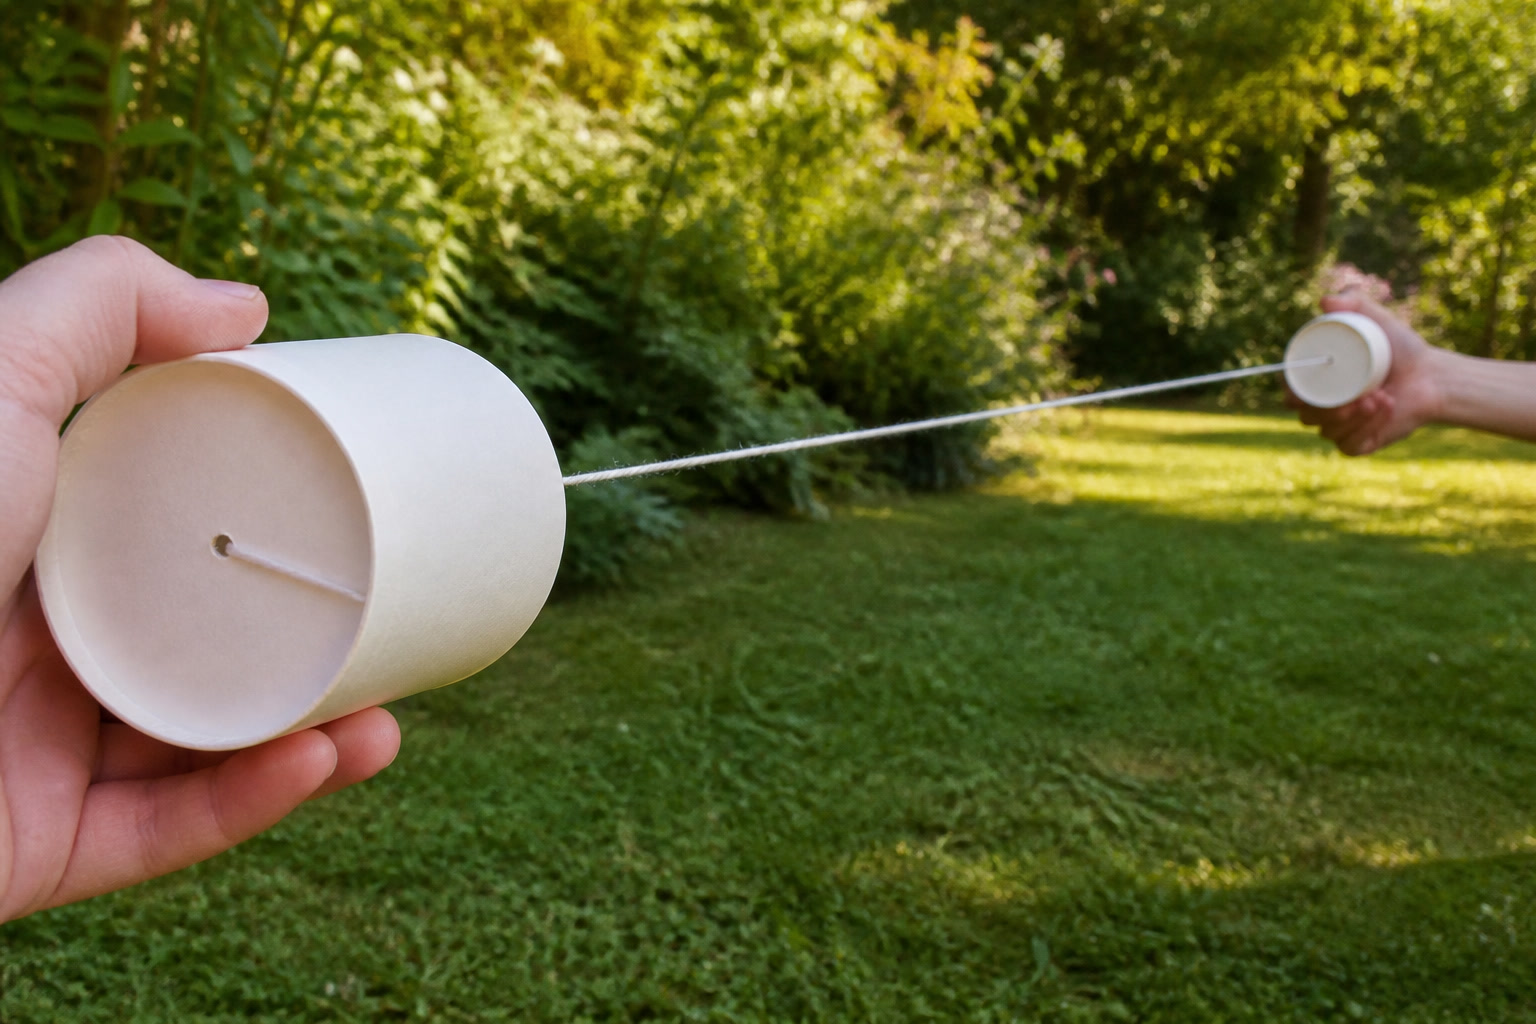
\includegraphics[width=0.58\linewidth]{images/book1/ai/g4-sound-string-telephone.jpg}

{\small डोरी वाला टेलीफ़ोन, कसकर तना हुआ: तनी हुई डोरी थरथराहट को एक कप से दूसरे कप तक उस \omterm{def:g2:air-around-us:air}{हवा} के मुक़ाबले कहीं बेहतर पहुँचाती है जो दो फुसफुसाने वालों के बीच होती है।}
\end{omfigure}

\section{ध्वनि समय लेती है}

\begin{proposition}[तेज़, पर पल भर में नहीं]\label{prop:g4:how-sound-travels:speed}
\omterm{def:g3:sound-around-us:sound}{ध्वनि} दौड़ने वाली है, जादूगर नहीं: \omterm{def:g2:air-around-us:air}{हवा} में वह हर सेकंड लगभग
\qty{340}{m} पार करती है --- यानी लगभग एक किलोमीटर के लिए तीन सेकंड।
\omterm{def:g1:light-and-shadows:source}{प्रकाश}, इसके उलट, इतनी तेज़ी से पहुँच जाता है कि जिस भी दृश्य को तुम
देख सको, उसके लिए उसका सफ़र पल भर का ही गिना जाता है। तूफ़ान की पूरी
कहानी इसी फ़र्क़ में है।
\end{proposition}

\begin{method}[तूफ़ान कितनी दूर है?]\label{met:g4:how-sound-travels:storm}
\begin{enumerate}
  \item कौंध दिखते ही बराबर ताल से सेकंड गिनना शुरू करो: एक मगरमच्छ,
        दो मगरमच्छ, \dots;
  \item बादल की पहली गड़गड़ाहट पर रुक जाओ;
  \item अपनी गिनती को $3$ से भाग दो: यही मोटे तौर पर तूफ़ान की दूरी
        किलोमीटर में है।
\end{enumerate}
छह सेकंड: लगभग \qty{2}{km}। कड़कों के बीच गिनती छोटी होती जाए तो
तूफ़ान पास आ रहा है --- भीतर चले जाने का समय।
\end{method}

\begin{omfigure}
\begin{tikzpicture}[scale=0.85]
  \draw[thick] (0,0) -- (11,0);
  \draw[very thick, omThm] (1.3,3.4) -- (0.9,2.5) -- (1.25,2.5)
    -- (0.8,1.5) -- (1.15,1.5) -- (0.7,0.4);
  \fill[omExo, opacity=0.3] (0.3,3.4) ellipse (1.5 and 0.45);
  % the listener, counting the silent seconds
  \fill (9.6,1.32) circle (0.18);
  \draw[thick] (9.6,1.14) -- (9.6,0.55);
  \draw[thick] (9.6,1.02) -- (9.33,0.75);
  \draw[thick] (9.6,1.02) -- (9.87,0.75);
  \draw[thick] (9.6,0.55) -- (9.4,0);
  \draw[thick] (9.6,0.55) -- (9.8,0);
  \foreach \r in {0.7, 1.4, 2.1} {
    \draw[omDef, thick] (1.0,0.4) ++(\r,0) arc (0:40:\r);
    \draw[omDef, thick] (1.0,0.4) ++(\r,0) arc (0:-12:\r);
  }
  \node[font=\small, align=center] at (9.15,2.35)
    {``\dots{}पाँच, छह''\\--- लगभग \qty{2}{km}};
  \node[right, font=\small, omDef] at (3.6,0.75)
    {गड़गड़ाहट, हर सेकंड \qty{340}{m} दौड़ती हुई};
\end{tikzpicture}

{\small कौंध अभी, गड़गड़ाहट बाद में: \omterm{def:g1:light-and-shadows:source}{प्रकाश} उसी पल पहुँच जाता है,
\omterm{def:g3:sound-around-us:sound}{ध्वनि} हर सेकंड \qty{340}{m} की चाल से दौड़ती है। सन्नाटे के सेकंड ही
दूरी माप देते हैं।}
\end{omfigure}

\begin{example}[प्रतिध्वनि]\label{ex:g4:how-sound-travels:echo}
मैदान के उस पार किसी बड़ी चट्टान या अकेली इमारत की ओर चिल्लाओ:
``हलो!'' --- पल भर का सन्नाटा --- ``हलो!'' तुम्हारी अपनी आवाज़ जवाब
देती है। \omterm{def:g3:sound-around-us:sound}{ध्वनि} बड़ी कठोर दीवारों से टकराकर लौटती है, और लौटी हुई ऐसी
\omterm{def:g3:sound-around-us:sound}{ध्वनि} जो इतनी देर से आए कि अलग से सुनी जा सके,
\emph{प्रतिध्वनि}\index{प्रतिध्वनि} कहलाती है। दीवार जितनी दूर,
तुम्हारी आवाज़ का चक्कर उतना ही लंबा, और \omterm{ex:g4:how-sound-travels:echo}{प्रतिध्वनि} उतनी ही देर से।
छोटे कमरे में लौटी हुई \omterm{def:g3:sound-around-us:sound}{ध्वनि} इतनी जल्दी आ जाती है कि अलग से सुनी ही
नहीं जा सकती --- वह बस तुम्हारी आवाज़ को भरा-भरा बना देती है।
\end{example}

\begin{remark}[सोनार: प्रतिध्वनि को काम पर लगाना]\label{rem:g4:how-sound-travels:sonar}
जहाज़ समुद्र की गहराई नीचे की ओर चिल्लाकर मापते हैं --- यानी पानी में
एक चटकी भेजकर --- और तल से लौटी \omterm{ex:g4:how-sound-travels:echo}{प्रतिध्वनि} का समय लेकर। गहरा पानी,
देर से \omterm{ex:g4:how-sound-travels:echo}{प्रतिध्वनि}; उथला पानी, जल्दी \omterm{ex:g4:how-sound-travels:echo}{प्रतिध्वनि}। डॉल्फ़िन और चमगादड़
यह तरकीब जन्म से जानते हैं: वे चटकी भेजते हैं और सुनते हैं, और
प्रतिध्वनियाँ पढ़कर अँधेरे पानी तथा घुप अँधेरी गुफाओं में शिकार करते
हैं। बादल की गड़गड़ाहट के सेकंड गिनकर तुम उनका तरीक़ा पहले ही काम में
ला चुके हो: \omterm{def:g3:sound-around-us:sound}{ध्वनि} का समय नापो, दूरी जान लो।
\end{remark}

\section{अभ्यास}

\begin{exercise}[$\star$]\label{exo:g4:how-sound-travels:1}
इस अध्याय से \omterm{def:g3:sound-around-us:sound}{ध्वनि} के तीन वाहक बताओ, और एक ऐसी जगह जहाँ \omterm{def:g3:sound-around-us:sound}{ध्वनि} सफ़र
कर ही नहीं सकती।
\end{exercise}

\begin{exercise}[$\star$]\label{exo:g4:how-sound-travels:2}
मर्तबान वाले प्रयोग में घंटी का हथौड़ा बजता रहता है और बजना मर जाता
है। ठीक-ठीक क्या छीना गया, और इससे क्या साबित होता है?
\end{exercise}

\begin{exercise}[$\star$]\label{exo:g4:how-sound-travels:3}
\omterm{def:g2:moon-in-the-sky:moon}{चंद्रमा} चुप दुनिया क्यों है? अध्याय की प्रतिज्ञप्ति से उत्तर दो।
\end{exercise}

\begin{exercise}[$\star$]\label{exo:g4:how-sound-travels:4}
डोरी वाले टेलीफ़ोन में फुसफुसाहट को कौन ले जाता है? टेलीफ़ोन चालू
रखने के दोनों नियम बताओ।
\end{exercise}

\begin{exercise}[$\star$]\label{exo:g4:how-sound-travels:5}
\omterm{def:g2:air-around-us:air}{हवा} में \omterm{def:g3:sound-around-us:sound}{ध्वनि} एक सेकंड में लगभग कितनी दूर जाती है? और तीन सेकंड में?
\end{exercise}

\begin{exercise}[$\star$]\label{exo:g4:how-sound-travels:6}
कौंध और गड़गड़ाहट के बीच तुम नौ सेकंड गिनते हो। तूफ़ान कितनी दूर है?
अगली कड़क पर तुम्हारा साथी सिर्फ़ तीन सेकंड गिनता है --- क्या बदला,
और तुम दोनों को क्या करना चाहिए?
\end{exercise}

\begin{exercise}[$\star$]\label{exo:g4:how-sound-travels:7}
मेज़ पर कान सटाने से वह खुरचन क्यों सुनाई दे जाती है जो \omterm{def:g2:air-around-us:air}{हवा} कभी
पहुँचा ही नहीं पाई?
\end{exercise}

\begin{exercise}[$\star$]\label{exo:g4:how-sound-travels:8}
\omterm{ex:g4:how-sound-travels:echo}{प्रतिध्वनि} क्या है? दूर वाली बड़ी चट्टान पास वाली से देर में जवाब
क्यों देती है?
\end{exercise}

\begin{exercise}[$\star$]\label{exo:g4:how-sound-travels:9}
जहाज़ का सोनार गहरे और उथले पानी में फ़र्क़ कैसे करता है? कौन-से दो
जानवर यही खेल खेलते हैं, और कहाँ?
\end{exercise}

\begin{exercise}[$\star\star$]\label{exo:g4:how-sound-travels:10}
पुरानी फ़िल्मों में खोजी लोग दूर आती रेलगाड़ी सुनने के लिए कान इस्पात
की पटरी से सटा लेते हैं। पटरी \omterm{def:g2:air-around-us:air}{हवा} से बहुत पहले रेलगाड़ी की चुग़ली क्यों
कर देती है? \omterm{def:g3:sound-around-us:sound}{ध्वनि} को पटरी से मिलने वाले दोनों फ़ायदे बताओ। (एक अच्छी
तरह ले जाने के बारे में है; दूसरे के लिए याद रखो कि पटरी सीधे
रेलगाड़ी तक जाती है, जबकि \omterm{def:g2:air-around-us:air}{हवा} में \omterm{def:g3:sound-around-us:sound}{ध्वनि} तालाब के छल्लों की तरह हर दिशा
में फैलती जाती है और फैलते-फैलते पतली पड़ती जाती है।)
\end{exercise}

\begin{exercise}[$\star\star$]\label{exo:g4:how-sound-travels:11}
किसी बड़े ख़ाली आँगन में खड़े होकर तुम एक बार ताली बजाते हो और पूरे
एक सेकंड बाद दूर की दीवार से अपनी ही ताली की चटाक लौटती सुनते हो।
\omterm{def:g3:sound-around-us:sound}{ध्वनि} उसी एक सेकंड में दीवार तक गई और वापस आई। दीवार कितनी दूर है ---
ध्यान रखो, पूरा चक्कर सोचना है!
\end{exercise}
